\section{Алгоритмическое обеспечение системы}

\subsection{Выявление необходимого представления в зависимости от запроса пользователя}

\subsubsection*{Общая характеристика}

В зависимости от типа запроса пользователя (обычный запрос веб-страницы или AJAX-запрос) могут отдаваться различные представления.
Также заказчики в различных субъектах России требуют свои особенности при отображении и формировании информации на странице.
Это также следует учитывать при расчёте имени представления.

Используемые обозначения:

\begin{easylist}
& ИП --– имя представления, которое запрашивает контроллер приложения. Это значение заполняется, если название представление отличается от названия действия контроллера.
& НД –-- название действия. Если оно не задано, то принимается как Index.
& ИР –-- имя региона. Например, для Ульяновска ИР будет Ulyanovsk, а для Владимира Vladimir.
& РП --– имя файла с представлением для определённого региона. Например, если существует представление ListOfContractors, то для Ульяновска будет ListOfContractorsUlyanovsk.
\end{easylist}

Суть алгоритма сводится к поиску необходимого представления, существующего в системе.

К примеру, существуют следующие представления: List, ListAjax, ListVladimir, ListUlyanovskAjax, Details.

Алгоритм для Ajax-запроса действия Details должен вернуть “Details”, а для действия List “ListAjax” для Владимира и “ListUlyanovskAjax” для Ульяновска.

При запросе не ajax-запросом действия List для Брянска и Ульяновска должно вернуться представление “List”, для Владимира “ListVladimir”.

\subsubsection*{Используемые данные}

\begin{easylist}
& имя региона, в котором развёрнута текущая копия программы. Данные берутся из файла конфигурации;
& контекст запроса, предоставляемый платформой ASP.NET MVC.
\end{easylist}

\subsubsection*{Результат выполнения}

Результатом выполнения алгоритма является имя файла с представлением, которое необходимо отобразить пользователю.

\subsubsection*{Логическое описание}

Логическое описание представлено на рисунке~\ref{img:algo-views}.

\begin{figure}[h!]
	\begin{center}
		\begin{minipage}[h]{\linewidth}
			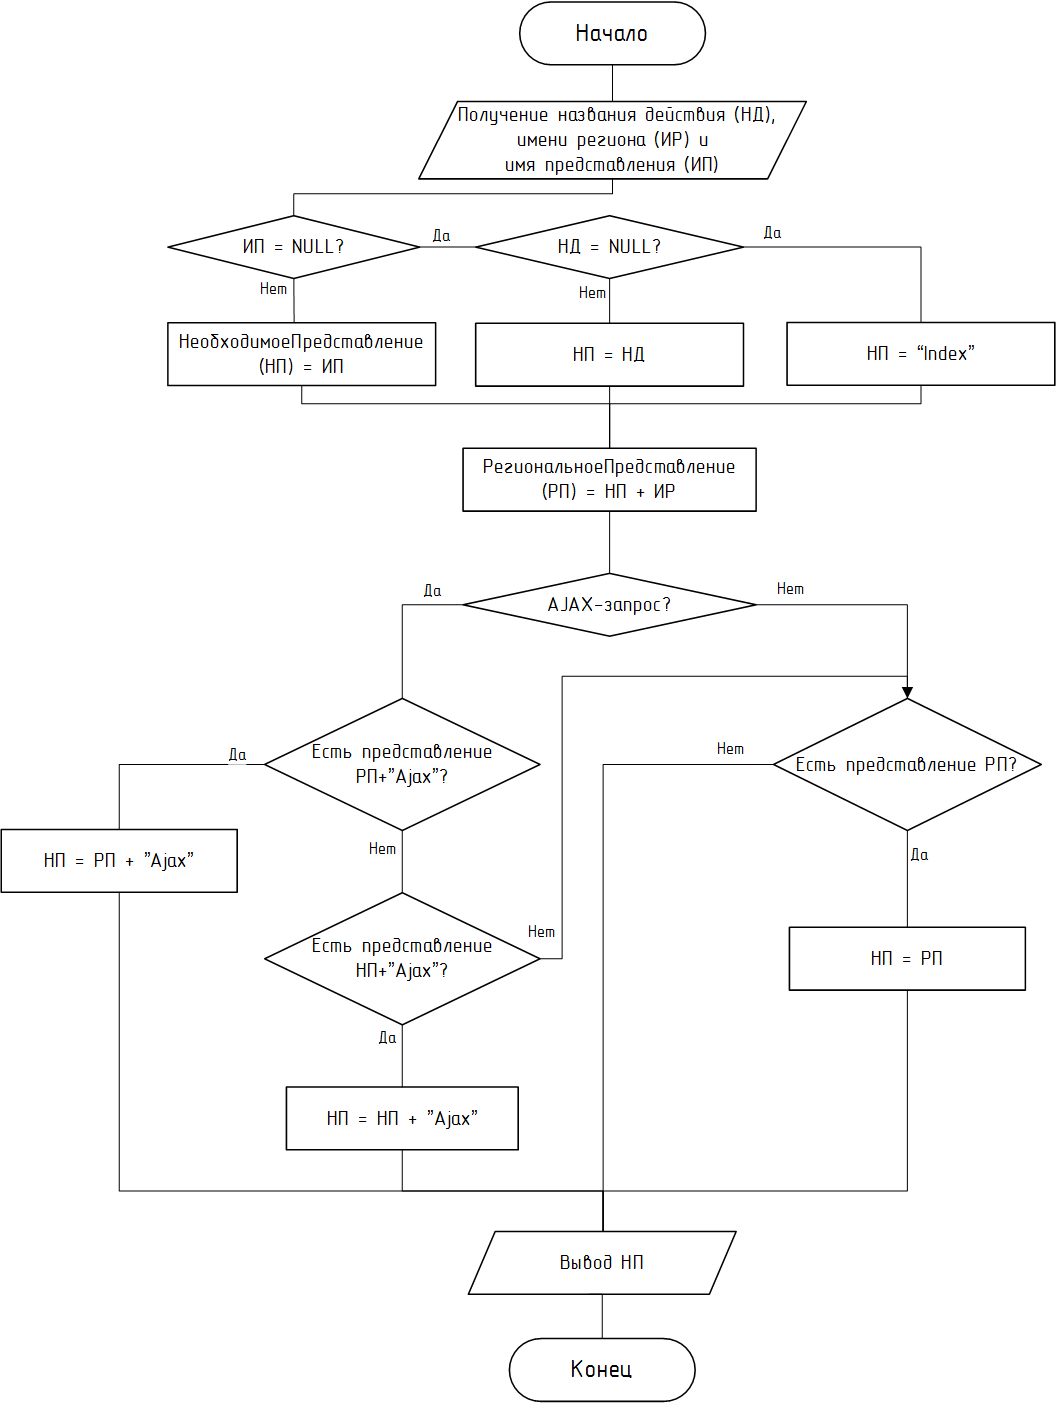
\includegraphics[width=\linewidth]{images/algo-views.png}
			\caption{Схема алгоритма расчёта имени представления}
			\label{img:algo-views}
		\end{minipage}
		\hfill
	\end{center}
\end{figure}  

\subsection{Авторизация пользователя при запросе к информационной системе}

\subsubsection*{Общая характеристика}

Информационная система должна отличать пользователей друг от друга.
Для этого придумано множество подходов.
Одним из них является авторизация пользователя по cookie, хранящегося на стороне клиента.
Cookie представляет собой определённую строку.

\subsubsection*{Используемые данные}

\begin{easylist}
& путь запроса пользователя;
& cookie-строка, содержащая информацию о сессии пользователя.
\end{easylist}

В ходе работы алгоритма используется транспорт с региональным сегментом системы ГИС ЖКХ от ООО <<АИС Город>>, в котором выполняются запросы к таблице cmn\$UserIndentity для получения из БД информации о пользователе.

\subsubsection*{Результат выполнения}

Результатом выполнения алгоритма является заполнение части контекста запроса пользователя, отвечающего за предоставление последнему прав и хранение информации о пользователе.

\subsubsection*{Логическое описание}

Логическое описание представлено на рисунке~\ref{img:algo-authorize}.

\begin{figure}[h!]
	\begin{center}
		\begin{minipage}[h]{\linewidth}
			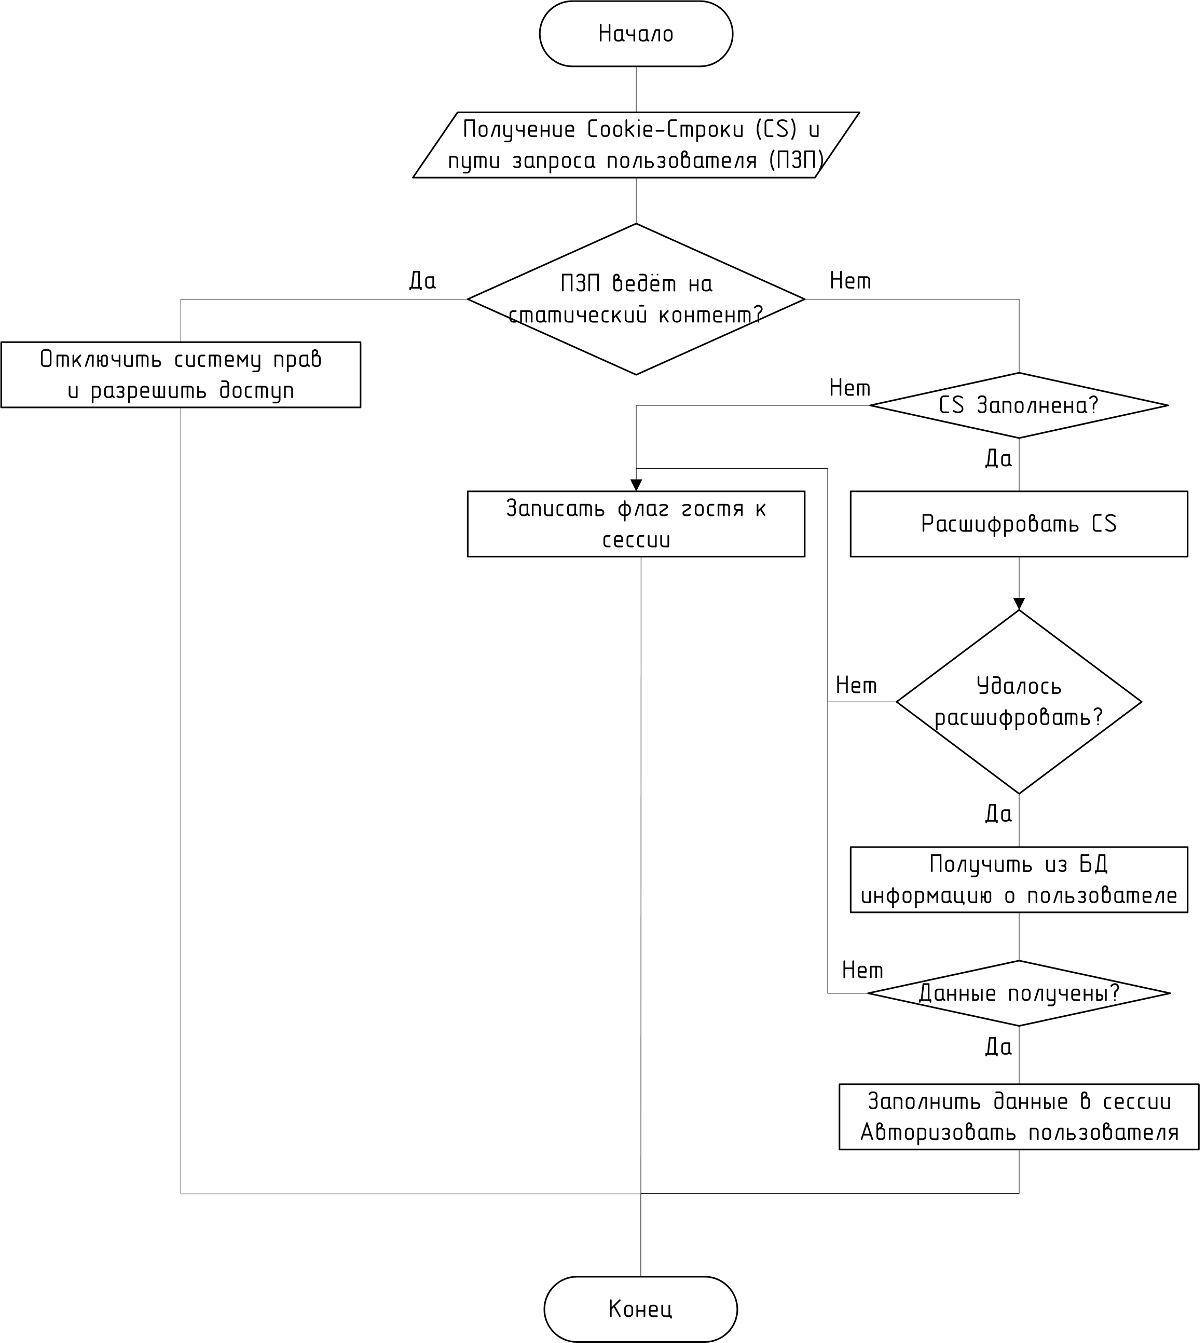
\includegraphics[width=\linewidth]{images/algo-authorize.png}
			\caption{Схема алгоритма авторизации}
			\label{img:algo-authorize}
		\end{minipage}
		\hfill
	\end{center}
\end{figure}  

\subsection{Расчёт статуса конкурса}

\subsubsection*{Общая характеристика}

Для фильтрации конкурсов необходимо определить его статус.

\subsubsection*{Используемые данные}

Данные о дате начала приёма заявок, окончании приёма заявок, вскрытии конвертов. Эти сведения размещаются в таблице Contest.

Число лотов данного конкурса из таблицы Lot, в которых заполнено поле WonBid.

\subsubsection*{Результат выполнения}

Результатом выполнения алгоритма является строка с названием статуса конкурса.

\subsubsection*{Логическое описание}

Логическое описание представлено на рисунке~\ref{img:algo-conteststatus}.

\begin{figure}[h!]
	\begin{center}
		\begin{minipage}[h]{\linewidth}
			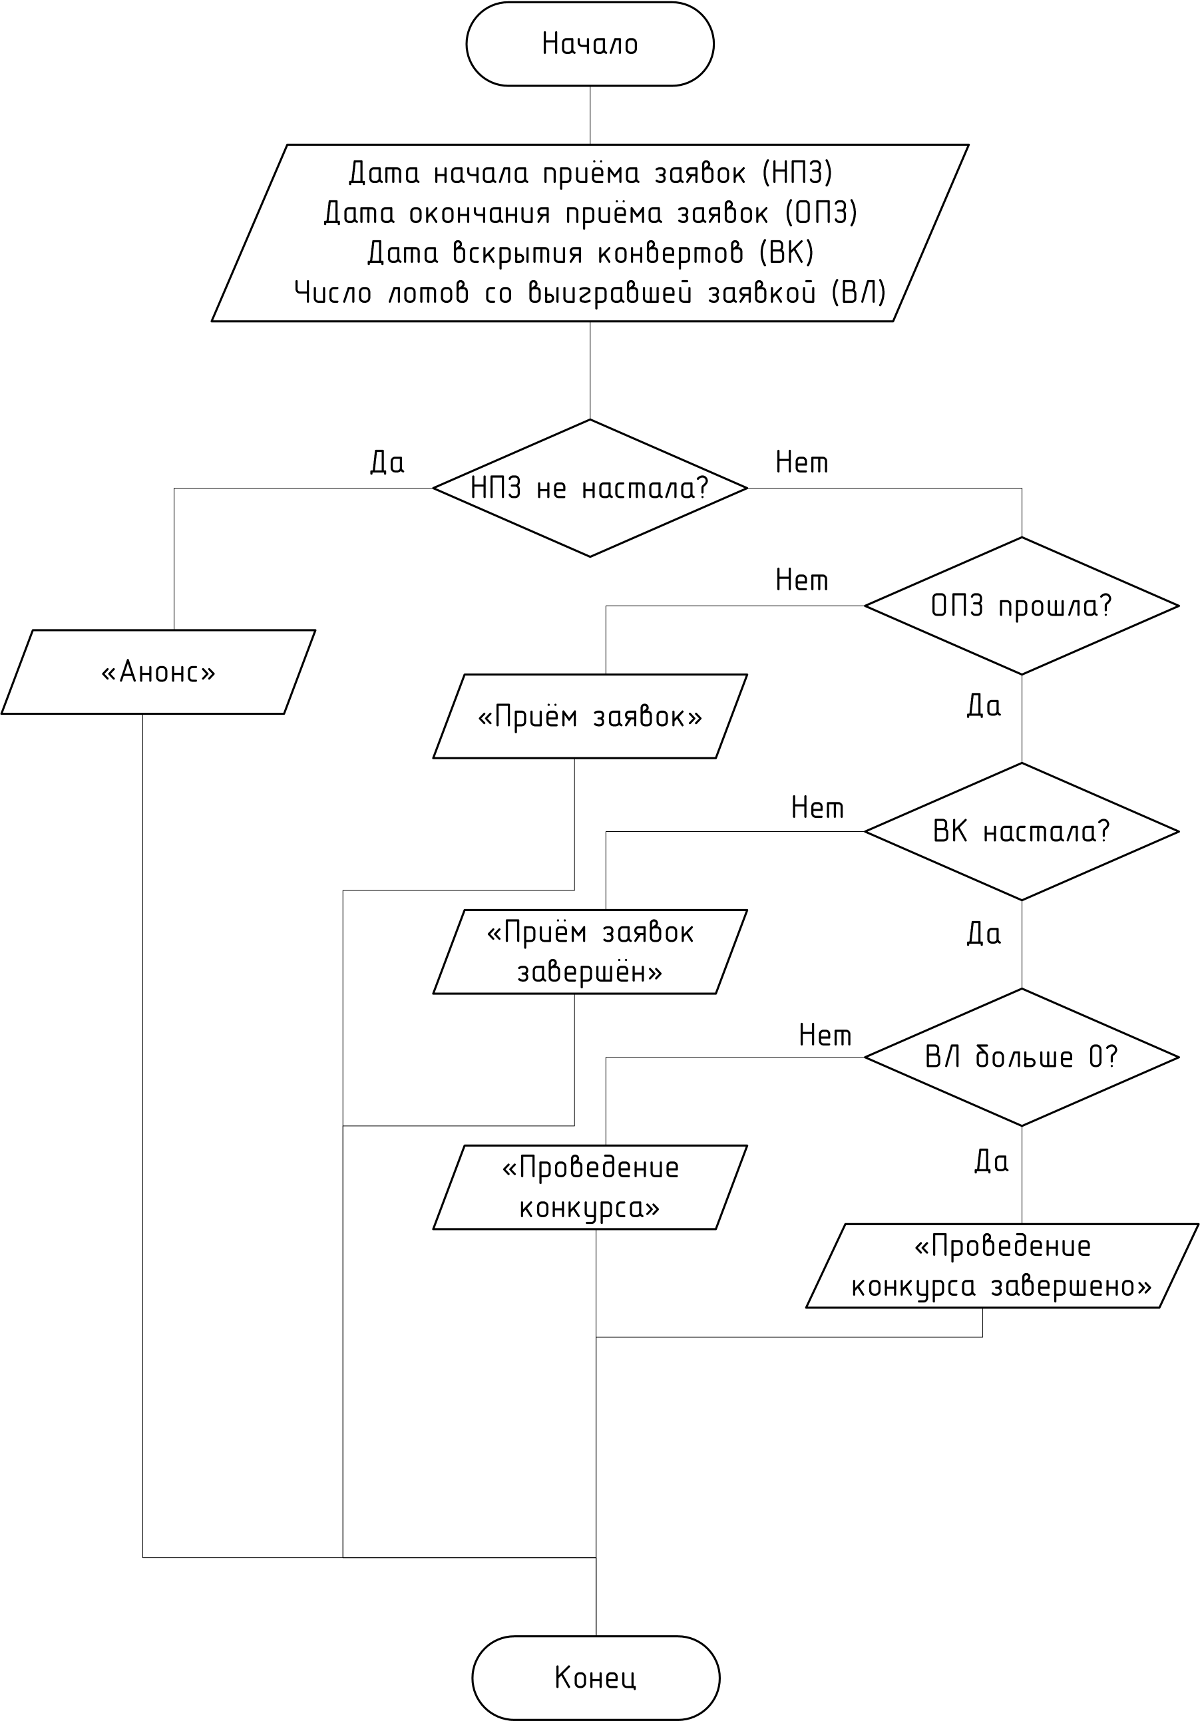
\includegraphics[width=0.8\linewidth]{images/algo-conteststatus.png}
			\caption{Схема алгоритма расчёта статуса конкурса}
			\label{img:algo-conteststatus}
		\end{minipage}
		\hfill
	\end{center}
\end{figure} 

\clearpage
\newpage